% THIS IS SIGPROC-SP.TEX - VERSION 3.1
% WORKS WITH V3.2SP OF ACM_PROC_ARTICLE-SP.CLS
% APRIL 2009
%
% It is an example file showing how to use the 'acm_proc_article-sp.cls' V3.2SP
% LaTeX2e document class file for Conference Proceedings submissions.
% ----------------------------------------------------------------------------------------------------------------
% This .tex file (and associated .cls V3.2SP) *DOES NOT* produce:
%       1) The Permission Statement
%       2) The Conference (location) Info information
%       3) The Copyright Line with ACM data
%       4) Page numbering
% ---------------------------------------------------------------------------------------------------------------
% It is an example which *does* use the .bib file (from which the .bbl file
% is produced).
% REMEMBER HOWEVER: After having produced the .bbl file,
% and prior to final submission,
% you need to 'insert'  your .bbl file into your source .tex file so as to provide
% ONE 'self-contained' source file.
%
% Questions regarding SIGS should be sent to
% Adrienne Griscti ---> griscti@acm.org
%
% Questions/suggestions regarding the guidelines, .tex and .cls files, etc. to
% Gerald Murray ---> murray@hq.acm.org
%
% For tracking purposes - this is V3.1SP - APRIL 2009

\documentclass{acm_proc_article-sp}
\usepackage{epstopdf}
\usepackage{graphicx}
\usepackage{amssymb, amsmath}
\graphicspath{{images/}}

\usepackage{subfig}
\usepackage[pdf]{pstricks}

\DeclareCaptionType{copyrightbox}

\captionsetup[figure]{position=t}
\captionsetup[subfigure]{position=b}
\usepackage[pdf]{pstricks}

\begin{document}

\title{A computational approach to understanding and predicting the behavior of educators using an online curriculum planning tool} 

%
% You need the command \numberofauthors to handle the 'placement
% and alignment' of the authors beneath the title.
%
% For aesthetic reasons, we recommend 'three authors at a time'
% i.e. three 'name/affiliation blocks' be placed beneath the title.
%
% NOTE: You are NOT restricted in how many 'rows' of
% "name/affiliations" may appear. We just ask that you restrict
% the number of 'columns' to three.
%
% Because of the available 'opening page real-estate'
% we ask you to refrain from putting more than six authors
% (two rows with three columns) beneath the article title.
% More than six makes the first-page appear very cluttered indeed.
%
% Use the \alignauthor commands to handle the names
% and affiliations for an 'aesthetic maximum' of six authors.
% Add names, affiliations, addresses for
% the seventh etc. author(s) as the argument for the
% \additionalauthors command.
% These 'additional authors' will be output/set for you
% without further effort on your part as the last section in
% the body of your article BEFORE References or any Appendices.

\numberofauthors{3} %  in this sample file, there are a *total*
% of EIGHT authors. SIX appear on the 'first-page' (for formatting
% reasons) and the remaining two appear in the \additionalauthors section.
%
\author{
% You can go ahead and credit any number of authors here,
% e.g. one 'row of three' or two rows (consisting of one row of three
% and a second row of one, two or three).
%
% The command \alignauthor (no curly braces needed) should
% precede each author name, affiliation/snail-mail address and
% e-mail address. Additionally, tag each line of
% affiliation/address with \affaddr, and tag the
% e-mail address with \email.
%
% 1st. author
\alignauthor
Ogheneovo Dibie \\
       \affaddr{University of Colorado }\\
       \affaddr{Institute of Cognitive Science}\\
       \affaddr{Dept. of Computer Science}\\
       \affaddr{Boulder, Colorado USA}\\
       \email{ogheneovo.dibie@colorado.edu}
% 2nd. author
\alignauthor
Keith Maull \\
\affaddr{University Corporation for Atmospheric Research }\\
\affaddr{Boulder, Colorado USA}\\
\email{kmaull@ucar.edu}
% 3rd. author
\alignauthor
Tamara Sumner \\
 \affaddr{University of Colorado }\\
\affaddr{Institute of Cognitive Science}\\
\affaddr{Dept. of Computer Science}\\
\affaddr{Boulder, Colorado USA}\\
       \email{sumner@colorado.edu}
}
% There's nothing stopping you putting the seventh, eighth, etc.
% author on the opening page (as the 'third row') but we ask,
% for aesthetic reasons that you place these 'additional authors'
% in the \additional authors block, viz.

% Just remember to make sure that the TOTAL number of authors
% is the number that will appear on the first page PLUS the
% number that will appear in the \additionalauthors section.

\maketitle
\begin{abstract}
In this paper, we present a computational approach to understanding and predicting the behavior of Earth Science educators using an online curriculum planning tool incorporating digital library resources. This paper expands on prior work on understanding educators' adoption and use of digital library resources \cite{maullunderstanding}. It introduces a methodology for characterizing user behaviors and understanding the trends and frequent patterns of use that are observable from these behaviors. Furthermore, we show that a user's behavior at the end of the school year can be predicted with an accuracy of 72.5\% from observing usage as early as the month of October
\end{abstract}

% A category with the (minimum) three required fields
\category{H.4}{Information Systems Applications}{Miscellaneous}
%A category including the fourth, optional field follows...
\category{D.2.8}{Software Engineering}{Metrics}[complexity measures, performance measures]

\terms{Theory}

\keywords{ACM proceedings, \LaTeX, text tagging} % NOT required for Proceedings

\section{Introduction}
In today's classroom, educational digital libraries play an important role of supporting educators in customizing their instruction to meet the diverse needs of students\cite{sumner:team}. 
They provide educators with high quality resources to supplement classic teaching materials such as textbooks and teaching guides. Also, digital libraries provide learners with avenues for informal learning--learning outside the classroom--as a way of augmenting knowledge and experiences gained in the classroom \cite{marchionini}. Given the importance of educational digital libraries to learning and teaching, it is necessary to improve our understanding of how resources within these libraries are used.  This knowledge would be beneficial in providing library providers and managers with information on how to support and improve the information needs of library patrons.

Understanding technology use spans far beyond the realm of digital libraries. In marketing science there has been extensive research into technology adoption and use. A  theoretical framework for understanding technology use is the use-diffusion framework proposed by Shih and Venkatesh \cite{shih2004beyond}.Use-diffusion characterizes the uses of a product in two dimensions: the frequency of use and variety of use \cite{shih2004beyond}.  For example, following the use-diffusion model, the usage patterns of Facebook users can be characterized based on the amount of time spent on the Facebook platform and the various types of actions performed during that time. Other theories of use consider a user's content preference in addition to usage frequency and variety \cite{brandtzaeg2010towards}. We discuss the use-diffusion as well as other paradigms of technology use in greater detail in section \ref{section:relatedwork}. 

Within the realm of digital libraries, recent research has focused on computational approaches for determining the usage behaviors of educators. Inspired by theories of technology use from Shih \& Venkatesh and Ram \& Jung \cite{shih2004beyond, ram1990conceptualization}, Maull et al. developed a use diffusion-based methodology for understanding how a group of middle and high school Earth Science educators used an online curriculum customization tool incorporating digital library resources \cite{maullunderstanding}. They generated a typology of user behaviors by clustering the clickstream of users. A user typology refers to the categorization of aggregate user behaviors into distinct user types \cite{brandtzaeg2010towards}. Each user type gives an overview of the manner of use of members of that type \cite{brandtzaeg2010towards}. For example a user of type \textit{power user} is one who spends a lot of time on a product and also uses it in a variety of contexts. Similar to the work of Maull et al. \cite{maullunderstanding}, Xu et al. studied the different  user types that emerged from teacher use of an educational digital library service, the Instructional Architect \cite{xu}. 

While current usage theories give insight into user types, they do not account for the evolution of such behavior. For example, a user of the type \textit{power user} (spends a lot of time on a product and exercises most of its features) after a year of using a product, may not have exhibited this behavior from first use. We hypothesize that user behaviors as described by user types are not static but dynamic. In fact, Shih and Venkatesh posit a similar hypothesis in elaborating on user types they discover \cite{shih2004beyond}. In this research, we aim at shedding light on the evolution of a user type by understanding how the patterns of use that describe it change over time and what frequent patterns can be observed within it. Using a market-basket analysis \footnote{Market-basket analysis is a data mining technique used in detecting frequent patterns in data transactions} type approach to analyze the usage patterns within a user type, we get a better understanding of the unique patterns of use that exist within that type. This would help in understanding the correlations that occur between usage features within specific user types. For example, when a user of a type \textit{power user} spends a high or low amount of time on the system, what actions are they likely to be performing etc.

Furthermore, current research on digital library use is mostly retrospective, i.e. a user's behavior is determined after a set period of use. Studies \cite{maullunderstanding,xu} were based on a year of use. We can however go a step further by predicting a user's behavior based on knowledge of a user typology. This could be especially useful for new users of the system as it could help system providers/managers with information on how to better support their needs based on predicted behaviors. In our domain (educational digital library resources), this could mean implementing better professional development (PD) training or improving accessibility to resources. For example, if after a couple months of usage, a user's behavior is predicted as likely being of the type \textit{limited use} (spends very little time on the system and likely to discontinue use), efforts could be made to encourage use or at least understand why the product is barely being used. In this paper, we develop computational models for predicting the long-term behaviors of users from small windows of time. We posit long term behavior as a user's membership in a user type at the end of our observation period--one academic year. 

The rest of this paper is organized in the following manner. In section 2, we discuss theoretical models and computational approaches for determining and predicting technology use. We state our research questions and the context for this study in sections 3 \& 4. Sections 5-8 highlight our approach and the results of our research studies addressing the questions posed in section 3. Section 9 discusses the limitations of this work and in section 10 we discuss its ramifications and future direction.
 
\section{RELATED WORK} \label{section:relatedwork}
This research draws upon theoretical models and computational approaches of determining technology use. We examine these theories in this section
\subsection{Theoretical models of technology use}
Technology use research follows from a rich history of work in technology adoption. Technology adoption occurs when a user decides an innovation is of utility and decides to use it \cite{straub2009understanding}. Most research on technology adoption is focused on factors that influence a user's decision to adopt an innovation. They include Roger's innovation diffusion theory where the five "adopter categories", a user's propensity to adopt an innovation and the spread of that innovation within a social system are examined \cite{rogers2010diffusion}. Other models of technology adoption include the concerns based model which focuses on an an individual's specific reasoning behind adopting an innovation \cite{fuller1975concerns, hall1979concerns} and the technology acceptance model \cite{legris2003people} which takes into account the influence of an individual's self efficacy and expertise in deciding whether to adopt a technology or not \cite{legris2003people}.

However technology adoption models do not account for how a technology is being used. Knowledge of how a product is used or not being used is key for producers in making improvements to the product. This need has led to the rise of theories that explain actual technology use.

A key theory on technology use is the theory of use-diffusion. Originally proposed by Ram and Jung\cite{ram1990conceptualization}, it measures technology use on two dimensions: frequency and variety. Usage frequency refers to how often a product is being used while variety refers to the different applications or contexts within which a product is being used. For example, usage frequency for an Ipad will be based on how long it is being used while usage variety encompasses the various applications it is used for e.g. games, word processing, camera etc.

The work of Ram and Jung was expanded on by Shih and Venkatesh \cite{shih2004beyond}.  Through self-report questionnaires and a diary study \footnote{A diary study is a study method common in the fields of anthropology, psychology and Human Computer Interaction (HCI) in which users log their interactions with a product. It provides a great way for researchers to context longitudinal data on a user's experience with a product.}of individuals using a household technology, they discover a user typology of four distinct user types: \textit{intense use, non-specialized use, specialized use, and limited use}.
Users of type \textit{intense use} are characterized by high frequency and a high variety of use. Users of type \textit{specialized use} are characterized by a high frequency but a low variety of use. An example of this could be an administrative assistant who spends a lot of time on a computer but only uses it for processing word documents. Users of type \textit{limited use} are characterized by low frequency and variety of use. Users of type \textit{Non-specialized use} are characterized by a high variety of use and low frequency.

\subsection{Computational approaches for determining user typologies}
Recent research has focused on extending theoretical foundations on user typologies to educational contexts. Rather than determining user types solely based on self-reported usage as is the case in \cite{shih2004beyond,ram1990conceptualization}, these computational approaches generate a typology of user behavior via clustering of actual usage. Clustering is a data mining technique for automatically grouping related items into bins. Clustering algorithms normally group data based on two measures: the similarity between the data objects within the same cluster (minimal intra-cluster distance), and the dissimilarity between the data objects of different clusters (maximal inter-cluster distance) \cite{han2006data}. Xu \cite{xu} examined the use of clustering techniques to generate fine grained user typologies within a web based instructional tool known as the Instructional Architect (IA). The IA is an educational digital library service designed to facilitate the creation of simple instructional projects using web resources from the National Science Digital Library (NSDL) and the web in general[9]. Projects created can be kept as private, shared with just students and other teachers or made publicly available on the web. Three clusters of users were discovered namely: key brokers, insular classroom practitioners and ineffective islanders \cite{xu}.  Key brokers frequently browsed projects created by other users in IA and their own projects also received a lot of attention from other users; their public projects were of high quality \cite{xu}.Insular classroom practitioners did not create high quality projects because their projects were characterized by very little content and links to external resources. They had little interest in viewing projects created by other IA users and most of the projects they created were limited to use with students in their classrooms. Ineffective islanders were characterized by publishing a single project of supposedly good quality but these projects were not shared with neither students nor the public \cite{xu}.

Working with the Curriculum Customization Service (CCS)--an online curriculum planning tool incorporating digital library resources \cite{sumner:team}, Maull et al. \cite{maullunderstanding} develop a typology of user behaviors observed in the CCS. This typology is inspired by a use-diffusion based  methodology and characterizes use based on  frequency and variety type metrics observable through server usage logs. Frequency based metrics include the number of session and hours spent, while variety based metrics include areas of the CCS that were accessed such as interactive resources, publisher materials, and user-contributed resources. We provide detailed explanation of these features in section 4. 

Our work is based on the same context as Maull et al \cite{maullunderstanding}. It extends their use-diffusion based methodology of understanding technology use in the following ways: 
\begin{enumerate}
\item This work provides an understanding of how usage features that characterize user types trend within the time period of the observed user type. A user type is defined by the values of a set of usage features (described in section \ref{usagefeaturesection})

\item This work introduces a market-basket analysis of usage features to understand what features are likely used in concert per user type. This answers the question of when users of type Y are doing X, what else are they likely to also be doing.

\item This works explores computational models to predict an educator's behavior from small time windows of usage data. It aims to provide understanding of the earliest time window of usage data and usage
\end{enumerate}

\subsection{Predicting User Behavior}
Predicting user behavior on the web has been of major research interest in recent times. This is primarily due to the need to improve user experience.  Research studies have looked into the correlation between  the online activities of users in order to understand how one influences the other \cite{adar2007we}. For example, this could be the likelihood a user purchasing an item after reading reviews or a blog post about it \cite{adar2007we}. Other research have explored online user behavior at a much lower level of granularity such as the likelihood of a user clicking on a sponsored search result \footnote{Sponsored search results are advertisements displayed by search engines next to the actual search results returned. They are major revenue source for most web search engines.} \cite{Attenberg:2009}. Attenberg et al. \cite{Attenberg:2009} show that a user's click through behavior on sponsored search results can be predicted with a decent degree of accuracy based on the user's search query,result and prior behavior. User behavior on sponsored search result is determined by the number of additional clicks made and time spent on sponsored results.

In this paper, we aim at exploring user behavior prediction in the context of an online planning tool incorporating digital library resources. We aim at identifying the most predictive features of a user's eventual user type and the earliest window of time within which a user's behavior can be accurately predicted.

\section{RESEARCH QUESTIONS}
The specific research questions to be addressed in this paper are as follows:
\begin{enumerate}
\item Does the usage pattern which describe a user type remain the same or does it vary and if so how?
\\In this question we examine how the value of usage features that describe a user type change from time to time
\item What are the frequent patterns of use that can be observed within a user type?
\\This question gets at what usage features go together within a particular user type. It would provide a better understanding of what users of a particular type are likely doing when doing something else.
\item How well can computational models predict a user's eventual user type from smaller time windows?
\\We examine a set of classifiers for predicting the user type of users at the end of a school year from earlier time frames such as
the first month of use and first semester of use. We aim to discover what time frame and usage features are best predictive of a user's user type
\end{enumerate}


\section{RESEARCH CONTEXT}
\label{researchcontext}
\begin{figure}
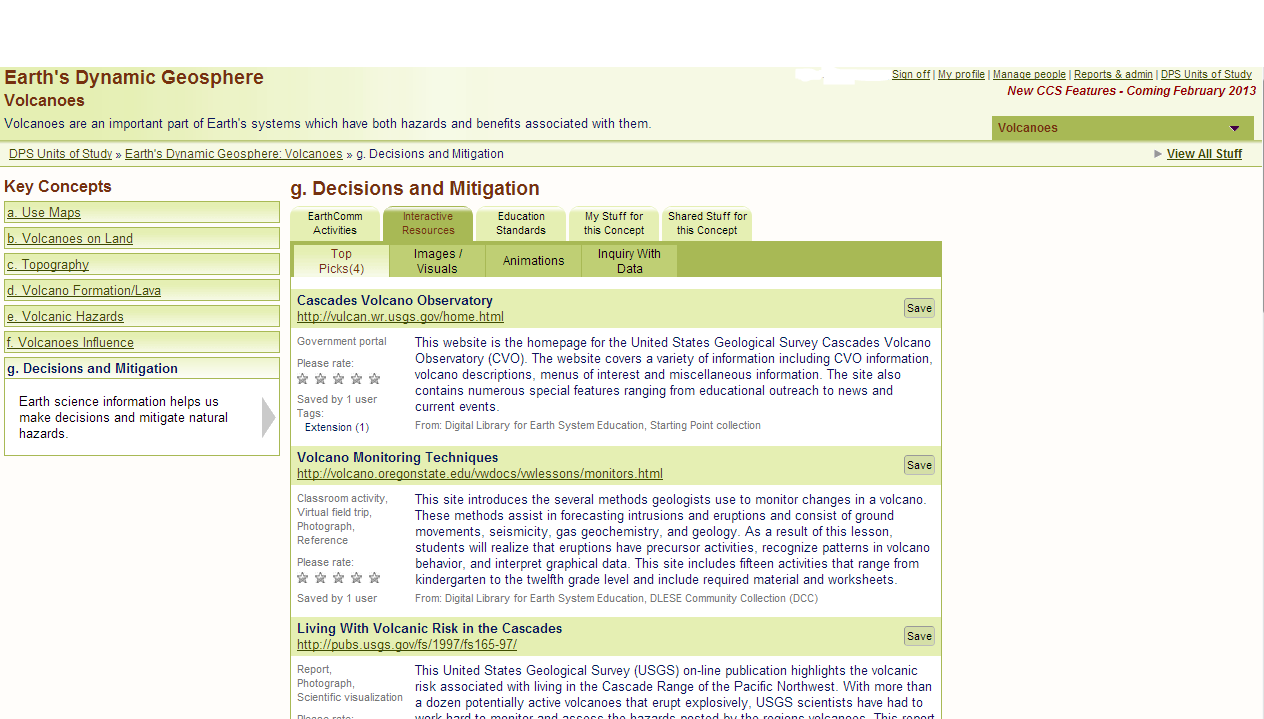
\includegraphics[width=1 \linewidth]{./ccsimage}
\caption{Snapshot of the CCS platform highlighting its main capabilities: Publisher materials (EarthComm Activities tab), Digital library resources (Interactive Resources tab), personalization capabilities(My Stuff tab) and community features (Shared stuff tab). The Interactive Resource tab is opened in this figure showing the top recommended digital resources}
\label{fig:ccsimage}
\end{figure}

The research questions outlined in this paper will be examined in the context of an instructional curriculum planning tool called the Curriculum Customization Service (CCS) \cite{sumner:team}. The CCS is a web based instructional planning tool which provides primarily middle and high school Earth Science teachers with access to digital versions of their class room text book, curriculum-relevant high quality, digital library resources and community-contributed resources. These resources are used in a multitude of pedagogical scenarios: from lesson planning to in-class projection and demonstration to customizing instruction to meet the needs of a diverse group of learners \cite{Saldivar:2012}. Educators use the CCS as a supplement to other instructional aids such as text books, teaching guides and other electronic resources. Deployed since the fall of 2009, the CCS is now being used in six school districts in the states of Colorado, Nevada and Utah. 

The CCS is instrumented to capture the click actions of users. Click actions being tracked include all unique page elements such as clicks on links, toggles, tabs, and buttons. The aggregate data collected from the clicking activity of users is collectively known as clickstream. Clickstream data is not only useful in showing a user's navigational path i.e. pages clicked on during a visit to a website, and click actions performed within a specific page (i.e. page elements that were clicked on within a particular page), but also a user browsing behavior \cite{montgomery2004modeling}. Clickstream analysis has proved to be very useful in developing user typologies from online usage as illustrated by Maull et al. \cite{maullunderstanding} with the CCS and Xu et al.\cite{xu} with the Instructional Architect. The clickstream data under analysis for this research includes information such as the user identity (user id), time stamp, specific system components clicked on (within the CCS this could be an interactive resource from a digital library such as DLESE or a user-contributed resource) and session length. A series of clicks performed over a period of time constitutes a session and a session is delineated by 45 minutes of inactivity or by the user logging out.

The CCS features four core areas: (1) Digital library resources, (2) Publisher material, (3) Community contributed resources and (4) Personalization. We briefly explain the purpose behind each of these areas below.
 
\textbf{Digital library resources}:
A core aim of the CCS is to enable users customize instruction with high-quality digital library resources. The CCS is designed to automatically pull educational resources from digital libraries such as the Digital Library for Earth System Education (DLESE) and align these resources to a curriculum and educational standards. Within the CCS' interface, these resources are collectively referred to as interactive resources(IR resources). IR resources are sub-grouped into four categories depending on its type as indicated in figure \ref{fig:ccsimage}. They are: Top Picks, Animations, Images/Visuals and Inquiry with Data. 

\textbf{Publisher materials}:
Publisher materials are digitized versions of primarily paper-based instructional materials. Publisher materials include a digitized version of the student textbook, and supplemental teaching materials such as instructional support materials, teaching tips and embedded assessments. Access to digitized version of classic teaching materials within the CCS makes curriculum planning and in-class usage more accessible and convenient.

\textbf{Personalization}:
The CCS provides a host of personalization features which we refer to as \textbf{My Stuff}. As users go through the CCS platform, they can save publisher materials, digital library and community-shared resources to their My Stuff area. In addition to saving other system components, users can also upload their own resources to My Stuff and retrieve as needed at a later time.

\textbf{Community Features}:
The CCS promotes social behavior such as sharing resources among users. Within each section of the curriculum, users are able to share resources such as documents, links and rich media with others. Other users who find these resources useful can use or save these resources in My Stuff for later use.

\subsection{Data}
Our analysis is based on the clickstream of a large urban school district with 80 science educators which used the CCS during the 2011-2012 school year. About 20,000 click actions were registered by members of this district. We restrict our data set to the usage logs of all users during the months of September-May. Typically, the school calendar runs from August-June, but usage in August and June are partial as school begins in late August and ends in early June. Thus, we omit them from our analysis.

\subsubsection{Feature selection}\label{usagefeaturesection}
Our study is based on six usage features highlighted in table \ref{usagefeatures}. These features cover the four core areas of the CCS referred to in section \ref{researchcontext} and were used in clustering experiments by Maull et al \cite{maullunderstanding}. The total number of sessions and hours spent (features 1 \& 2) represent frequency based features while total activity within my stuff, publisher materials, shared stuff and interactive resources are variety based features. 

\section{CHARACTERIZING USER TYPES}\label{charusertypes}

\begin{table}

\centering
\caption{CCS usage features that characterize a user type.  }
\label{usagefeatures}
\begin{tabular}{|c|p{6.75cm}|} 
\hline
Num & Feature \\ \hline
1 & Total number of sessions (Num Sess) \\ \hline
2 & Total number of hours spent on the site (Hrs) \\ \hline
3 & Total "My Stuff" activity (MS Act) \\ \hline
4 & Total activity within publisher material (Pub Actv)\\ \hline
5 & Total Shared stuff activity (SS Actv) \\ \hline
6 & Total Interactive Resources activity (IR Act)	\\ \hline
\end{tabular}
\end{table}
Before proceeding with our analysis on understanding and predicting user types, we introduce the idea of discretizing the values of the usage features under analysis (see table \ref{usagefeatures}) into equal frequency bins of high, medium and low. Equal frequency binning provides a distribution-dependent notion of levels and avoid large frequency skews common in naive binning approaches \cite{han2006data}.

 To illustrate this consider the set of usage features \{Number of sessions, Hours spent, Interactive Resource Activity, My Stuff Activity, Shared Stuff Activity, Publisher Material Activity \} with values $\{20,4,90,23,45,55 \}$ that define a user's aggregate usage at the end of an observation period. The feature set here indicates that the user spent 4 hours on the platform across 20 sessions and performed 90,23,45 and 55 click actions within the interactive resources, my stuff, shared stuff and publisher material areas of the system respectively. A discretized value for each feature e.g. $\{high,mid,mid,low,low, mid\}$ gives an idea of how a user's usage compare to other users within the same observation period. Thus, a value of high in the number of sessions feature, indicates this user was in the high range compared to other users.
 
 Discretized feature values inform our characterization of clusters generated from  clustering experiments of usage  with user types, trend analysis of usage features, understanding of frequent patterns of use and prediction of user types. 
 

We generate a typology of user types as follows:

\begin{table}
\caption{Discretized feature values for aggregate usage data across all users during the 2011-2012 school year}
\label{aggfeaturebins}
\begin{tabular}{|p{3.5cm}|l|l|l|} 
% Add cluster label for cluster columns here
\hline
& \multicolumn{3}{c|}{\textbf{Bins}}  \\ \hline
\textbf{Feature} & Low & Mid & High \\ \hline
Num sess & -inf-6.5 & 6.5-20.5 & 20.5-inf \\ \hline
Hrs & -inf-0.89 &0.89-3.67 & 3.67-inf \\ \hline
IR Actv & -inf-0.5 & 0.5-14.5 & 14.5-inf \\ \hline
MS Actv & -inf-0.5 & 0.5-4.5 & 4.5-inf \\ \hline
SS Actv & -inf-2.5 & 2.5-17 & 17-inf \\ \hline
Publisher Activity & -inf-9 & 9-30.5 & 30.5-inf \\ \hline
\end{tabular}
\end{table}

\begin{enumerate}
\item The aggregate value for each usage feature across all users is discretized into equal frequency bins of high, medium and low as illustrated in table \ref{aggfeaturebins}.

\item We use the five user types discovered by Maull et al. \cite{maullunderstanding} and their discretized feature values as user type archetypes for characterizing usage as illustrated in table \ref{maull_features}. In table \ref{maull_features}, Cluster 1 refers to the \textbf{Limited use} ``uninterested adopter'' category. Members of this category have very low overall use of the CCS. Cluster 2 refers to the \textbf{Specialize use} ``Interactive Resource specialists.'' Members of this category make heavy use of interactive resources relative to other system features. Cluster 3 refers to the \textbf{Intense use} ``Ardent Power User'' category. Members of this group feature heavy robust use of all system features. Cluster 4 is the \textbf{Non-Specialized Use} ``Moderate Generalist'' category. They exhibit moderate overall system use. Cluster 5 is the \textbf{Specialized Use} ``Community Seeker Specialist'' category. They make heavy use of shared stuff and interactive resources relative to publisher materials

\item The EM algorithm is run against the total aggregate usage of all users to generate unique clusters. The output of EM clustering is a set of clusters (user types) with the cluster's mean value for each feature. We use the bin intervals discovered in step 1 to map each cluster's feature value to low, medium or high.

\item Finally, we attempt a mapping of the discretized feature values of each cluster to the user type archetypes from Maull et al. \cite{maullunderstanding}. If a mapping to a user type does not exist, we introduce a new label that describes the cluster based on its feature values.


\end{enumerate}

\begin{figure}
\centering
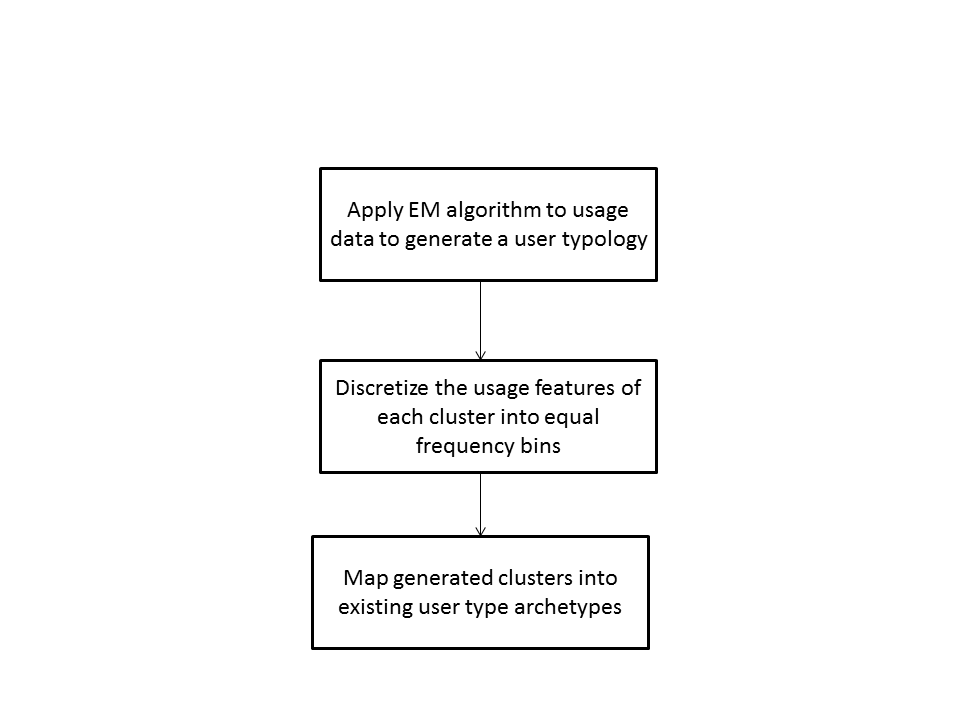
\includegraphics[width=1 \linewidth]{./process_flow}
\caption{Process flow of labeling a cluster with a user type}
\label{fig:process_flow}
\end{figure}

\begin{table}
\caption{Discretized feature values from cluster results of Maull et al. \cite{maullunderstanding}}
\label{maull_features}
\begin{tabular}{|p{2.5cm}|l|l|l|l|l|}
% Add cluster label for cluster columns here
\hline
& \multicolumn{5}{c|}{\textbf{Clusters}}  \\ \hline
\textbf{Feature} & 1 & 2 & 3 & 4 & 5 \\ \hline
Num sess & Low & Mid-High & High & High & High \\ \hline
Hrs & Low & Mid-High & High & High & High \\ \hline
IR Actv & Low & Low-mid & High & Mid & Low \\ \hline
MS Actv & Low & Mid-High & High & Mid & High \\ \hline
SS Actv & Low & High & High & High & High \\ \hline
Publisher Activity & Low & Low & High & Mid & Low \\ \hline
\end{tabular}
\end{table}


%\begin{table}
%\centering
%\caption{CCS usage features that characterize a user type}
%\begin{tabular}{|l|l|l|l|l|l|l|}} \hline
% User type & Number of sessions & Hours & IR_activity & Shared_stuff_activity & My_stuff_actv & Publisher_actv \\ \hline
%\textbf{Intense Use "Ardent Power User"} & High & High & High & High & High & High \\ \hline
%\textbf{Limited Use "Uninterested Non-Adopter"} & Low & Low & Low & Low & Low & Low \\ \hline
%\textbf{Specialized Use "Community seeker specialist"} & Mid-High & Low-Mid & Mid-High & High & Low & Low \\ \hline
%\textbf{Specialized use "Interactive resource specialist} & Mid-High & High & Low-Mid & Low-Mid & Low-mid \\ \hline
%\textbf{Non-specialized use "Moderage Generalist} & Mid & Mid & Mid & Mid & Mid & Mid \\ \hline
%\end{tabular}
%\end{table}

\subsection{User typology}

After clustering usage for all users we get a user typology as shown in table \ref{usertypology}
\begin{table}
\caption{Output of clustering experiments.The mean value of each feature is indicated in parenthesis}
\label{usertypology}
\begin{tabular}{|p{1.7cm}|p{1.6cm}|p{1.6cm}|p{1.6cm}|}
\hline
& \multicolumn{3}{c|}{\textbf{Clusters}}  \\ \hline
 \textbf{Feature} & 1 &  2 & 3 \\ 
\hline Num sess & Low(4.048)& High(97.2)  & High (26.5)  \\ 
\hline Hrs & Low (0.649) & High (17.802) & High (3.946)  \\ 
\hline IR Actv & Mid (3.867) & High (80.199) & High (18.275) \\ 
\hline MS Actv &  Low(0.781)  & High (10.2) & High (9.645)  \\ 
\hline SS Actv  & Low(1.6524) & High(21.6) & High(39.6) \\
\hline Pub Actv & Low(6.438) & High (162) & High (40.045)  \\
\hline \textbf{$N$} & 32 & 5 & 43 \\
\hline
\end{tabular}
\end{table} 

There were three clusters generated by the EM clustering algorithm. The number of clusters was decided using v-fold cross validation \footnote{In our case, v-fold cross validation works by setting the number of clusters to starting seed value of 1. The training set is split randomly into 10 folds. EM is performed across all folds sets and the loglikelihood is averaged over all 10 results. If the loglikelihood has increased the number of clusters is increased by 1 and the training set is split into another random 10 folds.}. We describe them as follows:

\textbf{Cluster 1}: With all its features with a value of \textit{Low} apart from interactive resources with a value of \textit{Mid}, this cluster is closest to the user archetype of limited use ``uninterested adopter.'' An introspection into the login frequency of members of this type, reveals that a good portion of users stopped using the CCS after the first few months of the school year.

\textbf{Cluster 2}: The usage pattern of cluster 2 with all feature values having a value of high is most closely related to the power user archetype.

\textbf{Cluster 3}: This cluster of users also have a high rating on average in all usage features. However, the values of each of these features are in the low range of the high value bin. On average users in this clusters are not as intensely engaged with the CCS platform as the power users in cluster 2. We would categorize these users as Community Seeker specialists, because they feature higher use of shared stuff compared to users of the other two clusters (in terms of mean number of clicks).

\section{USAGE PATTERN TRENDS}
We explore the trend in usage pattern on a feature-by-feature basis. In this analysis we look into how the mean values of each usage feature per user type changes on three levels: semester to semester, every two months and month to month. This would give a good idea of which usage features remain relatively stable (in terms of use) and which vary per user type. This knowledge would be particularly useful in detecting strong features that define a user type. For example, if the power user type always has a high value in  publisher material activity, this  might indicate that a high value in publisher material activity is a strong predictor of a power user.
\subsection{Limited use user type}
\subsubsection{Semester-Semester trends}
\begin{table}
\caption{Usage feature values of during the fall \& spring semesters of the `Limited use' user type}
\label{cluster0semester}
\begin{tabular}{|p{1.4cm}|p{0.6cm}|p{0.6cm}|p{0.6cm}|p{0.6cm}|p{0.8cm}|p{0.8cm}|}
\hline
& \multicolumn{6}{c|}{\textbf{Usage features}}  \\ \hline
 \textbf{Period} & Num sess & Hrs & IR Actv & MS Actv & Pub Actv & SS Actv \\ \hline
 Fall  semester & Low & Low  & Mid & Mid & Low & Low \\ \hline
Spring semester & Low & Low  & Mid & Mid & Low & Low \\ \hline
\end{tabular}
\end{table}
According to table \ref{cluster0semester}, all usage feature values remain the same across both semesters. This indicates that the mean usage among members of this group is stable across semesters.
\subsubsection{Bi-monthly trends}
\begin{table}
\caption{Bi-monthly usage feature values of the `Limited use' user type.}
\label{cluster0bimonthly}
\begin{tabular}{|p{1.5cm}|p{0.6cm}|p{0.6cm}|p{0.6cm}|p{0.6cm}|p{0.8cm}|p{0.8cm}|}
\hline
& \multicolumn{6}{c|}{\textbf{Usage features}}  \\ \hline
 \textbf{Period} 
 & Num sess & Hrs & IR Actv & MS Actv & Pub Actv & SS Actv \\ \hline
Sept-Nov & Low & Low  & Mid & Mid & Mid & Mid \\ \hline
Nov-Jan & Low & Mid  & Mid & Low & Mid & Low \\ \hline
Jan-Mar & Low & Mid  & Mid & Mid & Low & Mid \\ \hline
Mar-May & Low & Low  & Mid & Low & Low & Mid \\ \hline
\end{tabular}
\end{table}
To further investigate changes in the usage feature values, we considered mean values of these features on a bi-monthly basis as indicated in table \ref{cluster0bimonthly}. Like our semester-semester analysis, the number of sessions and interactive resource activity remains stable across all four time windows.  However, activity in my stuff, publisher material and shared stuff  varies between the mid and low value ranges. 
\subsubsection{Monthly trends}
\begin{table}
\label{cluster0month}
\caption{Monthly usage feature trends in the limited use user type}
\begin{tabular}{|p{1.2cm}|p{0.7cm}|p{0.7cm}|p{0.7cm}|p{0.7cm}|p{0.8cm}|p{0.8cm}|}
\hline
& \multicolumn{6}{c|}{\textbf{Usage features}}  \\ \hline
 \textbf{Month} 
 & Num Sess & Hrs & IR Actv & MS Actv & Pub Actv & SS Actv \\ \hline
\textbf{Sept} & Low                                    & Mid   & Mid         & Low             & Mid            & Low                 \\  \hline
\textbf{Oct}   & Low                                    & Mid   & Mid         & Low             & Low            & Mid                 \\  \hline
\textbf{Nov}  & Mid                                    & Mid   & Mid         & Low             & Mid            & Low                 \\  \hline
\textbf{Dec}  & Low                                    & Mid   & High        & Mid             & Mid            & Mid                 \\  \hline
\textbf{Jan}   & Mid                                    & Mid   & Mid         & Low             & Mid            & Low                 \\ \hline
\textbf{Feb}  & Mid                                    & Mid   & Low         & Low             & Mid            & Low                 \\  \hline
\textbf{Mar}     & Mid                                    & Low   & Mid         & Mid             & Mid            & Mid                 \\ \hline
\textbf{Apr}     & Low                                    & Mid   & Mid         & Low             & Mid            & Low                 \\ \hline
\textbf{May}       & Low                                    & Mid   & Low         & Low             & Low            &   Low              \\ \hline   
\end{tabular}
\end{table}
On a month-month basis, the hours spent and publisher activity features seem to be very stable and hence good predictors of membership within the limited use user type. The other features number of sessions, shared stuff activity and  interactive resource activity tend to vary quite a bit from month to month. This is illustrated in table \ref{cluster0month}

\subsection{Community Seeker user type}

\subsubsection{Semester-Semester trends}

\begin{table}
\caption{Usage feature values of the ``Community seeker'' user type of during the fall and  spring semesters}
\label{cluster2semester}
\begin{tabular}{|p{1.5cm}|p{0.6cm}|p{0.6cm}|p{0.6cm}|p{0.6cm}|p{0.8cm}|p{0.8cm}|}
\hline
& \multicolumn{6}{c|}{\textbf{Usage features}}  \\ \hline
 \textbf{Semester} 
 & Num sess & Hrs & IR Actv & MS Actv & Pub Actv & SS Actv \\ \hline
Fall  semester & High & Mid  & High & High & High & High \\ \hline
Spring semester & Mid & High  & Mid & High & High & High \\ \hline
\end{tabular}
\end{table}

As highlighted in table \ref{cluster2semester}, within the community seeker user type, activity in my stuff, shared stuff and publisher material remained at a high level on average. However, frequency based features (hours \& number of sessions) moved from the high-mid and mid-high level ranges respectively. This might indicate that users  spent less time across more sessions and more time across less sessions in the fall and spring semesters respectively. Also use of interactive resources dropped from high to mid from the fall to spring semesters

\subsubsection{Bi-monthly trends}
On a bi-monthly basis, the feature values of hours spent, interactive resource and publisher material activity remain fairly stable across all time windows. This could indicate the strength of these features in predicting membership within this class. The number of sessions, my stuff and shared stuff activity oscillate between the mid and high value ranges across the time chunks. This is illustrated in table \ref{cluster2bimonthly} 
\begin{table}
\caption{Bi-monthly usage feature values of the ``Community Seeker'' user type}
\label{cluster2bimonthly}
\begin{tabular}{|p{1.5cm}|p{0.6cm}|p{0.6cm}|p{0.6cm}|p{0.6cm}|p{0.8cm}|p{0.8cm}|}
\hline
& \multicolumn{6}{c|}{\textbf{Usage features}}  \\ \hline
 \textbf{Period} 
 & Num sess & Hrs & IR Actv & MS Actv & Pub Actv & SS Actv \\ \hline
Sept-Nov & Mid & Mid  & High & High & High & High \\ \hline
Nov-Jan & High & Mid  & Mid & Mid & Mid & Mid \\ \hline
Jan-Mar & Mid & Mid  & Mid & Mid & Mid & High \\ \hline
Mar-May & Mid & Mid  & Mid & High & Mid & High \\ \hline
\end{tabular}
\end{table}
\subsubsection{Monthly trends}
\begin{table}
\caption{Usage feature values on a month-month basis in the Community Seeker user type}
\label{cluster2month}
\begin{tabular}{|p{1.5cm}|p{0.6cm}|p{0.6cm}|p{0.6cm}|p{0.6cm}|p{0.8cm}|p{0.8cm}|}
\hline
& \multicolumn{6}{c|}{\textbf{Usage features}}  \\ \hline
 \textbf{Month} 
 & Num sess & Hrs & IR Actv & MS Actv & Pub Actv & SS Actv \\ \hline
\textbf{Sept} & Mid                                    & Mid   & Mid         & Mid             & Mid            & High              \\  \hline 
\textbf{Oct}   & Mid                                    & Mid   & Mid         & Mid             & Mid            & High               \\  \hline 
\textbf{Nov}  & High                                   & High  & High        & High            & Mid            & High              \\  \hline 
\textbf{Dec}  & High                                   & Mid   & Mid         & Mid             & Mid            & High            \\  \hline 
\textbf{Jan}   & High                                   & High  & High        & High            & High           & Mid                 \\  \hline 
\textbf{Feb}  & Mid                                    & Mid   & High        & High            & Mid            & High                 \\  \hline 
\textbf{Mar}     & High                                   & Mid   & High        & High            & Mid            & Mid                 \\  \hline 
\textbf{Apr}     & Mid                                    & Mid   & High        & High            & Mid            & High                \\  \hline 
\textbf{May}       & Mid                                    & High  & Mid         & Mid             & High           & Mid           \\  \hline       
\end{tabular}
\end{table}
Apart from the months of September and October where all usage features maintained the same values, the usage features tend oscillate between the mid and high value range bins as indicated in table \ref{cluster2month} .

\subsection {Power user user type}
Within the ``power user'' user type, usage features were examined in a semester-semester, bi-monthly and monthly basis.

\subsubsection{Semester-Semester trends}

\begin{table}
\caption{Usage feature values of during the spring semester of the ``Power User'' user type}
\label{cluster1semester}
\begin{tabular}{|p{1.5cm}|p{0.6cm}|p{0.6cm}|p{0.6cm}|p{0.6cm}|p{0.8cm}|p{0.8cm}|}
\hline
& \multicolumn{6}{c|}{\textbf{Usage features}}  \\ \hline
 \textbf{Semester} 
 & Num sess & Hrs & IR Actv & MS Actv & Pub Actv & SS Actv \\ \hline
Fall  semester & High & High  & High & High & High & High \\ \hline
Spring semester & High & High  & High & High & High & high \\ \hline
\end{tabular}
\end{table}

All usage features trend at a high level for members of the power user category during the fall and spring semester on average. This is similar to the trend overall during the entire school year. We examine these features on a deeper level to discover if any differences in the values of these features can be observed on a bi-monthly or monthly level.

\subsubsection{Trends every two months}
\begin{table}
\caption{Bi-monthly usage feature values of the ``Power User'' user type}
\label{cluster1bimonthly}
\begin{tabular}{|p{1.5cm}|p{0.6cm}|p{0.6cm}|p{0.6cm}|p{0.6cm}|p{0.8cm}|p{0.8cm}|}
\hline
& \multicolumn{6}{c|}{\textbf{Usage features}}  \\ \hline
 \textbf{Period} 
 & Num sess & Hrs & IR Actv & MS Actv & Pub Actv & SS Actv \\ \hline
Sept-Nov & High & High  & High & High & High & High \\ \hline
Nov-Jan & High & High  & High & Mid & High & High \\ \hline
Jan-Mar & High & High  & High & High & High & High \\ \hline
Mar-May & High & High  & High & Mid & High & Mid \\ \hline
\end{tabular}
\end{table}

Considering 2-month time frames as illustrated in table \ref{cluster1bimonthly}, all usage features maintain a value of high apart from My Stuff and Shared Stuff activities during the school year. My stuff activity dips between time periods of September-November and November-January and again from between time periods January-March and March-May.
My Stuff and Shared stuff activity dips to a Low value range from a high-value range during the time of periods of January-March and March-May.


\begin{table}[htbp!]
\caption{Usage features month-month in the Power User user type}
\label{cluster1month}
\begin{tabular}{|p{1.5cm}|p{0.6cm}|p{0.6cm}|p{0.6cm}|p{0.6cm}|p{0.8cm}|p{0.8cm}|}
\hline
& \multicolumn{6}{c|}{\textbf{Usage features}}  \\ \hline
 \textbf{Month} 
 & Num sess & Hrs & IR Actv & MS Actv & Pub Actv & SS Actv \\ \hline
\textbf{Sept} & High                                   & High  & High        & Mid             & High           & High                \\ \hline
\textbf{Oct}   & High                                   & High  & High        & High            & High           & Mid                 \\ \hline
\textbf{Nov}  & High                                   & High  & Mid         & Mid             & High           & Mid                 \\ \hline
\textbf{Dec}  & High                                   & High  & High        & Low             & High           & Mid                 \\ \hline
\textbf{Jan}   & High                                   & High  & High        & High            & High           & High                \\ \hline
\textbf{Feb}  & High                                   & High  & Low         & Mid             & High           & Mid                 \\ \hline
\textbf{Mar}     & High                                   & High  & High        & Mid             & High           & High                \\ \hline
\textbf{Apr}     & High                                   & High  & Mid         & Low             & High           & Low                 \\ \hline
\textbf{May}       & High                                   & High  & Low         & Low             & High           & Mid         \\  \hline     
\end{tabular}
\end{table}
\subsubsection{Monthly trends}
From table \ref{cluster1month}, it is clear that the number of sessions, hours and My Stuff Activity values retain a high value across all months. This indicates that a value of high in these three features is a strong predictor of membership within this cluster.  The values of interactive resource activity, My Stuff activity and shared stuff Activity vary quite a bit within the school year.

\section{FREQUENT PATTERNS OF USE}
The aim of this study is to understand what actions of members of a specific user type usually go together. As an example, we would like to understand what members of the ``power user'' user type are likely doing when they spend a high amount of time on publisher materials. This would give a good understanding of what usage feature correlations occur within a user type.

We take a market basket analysis approach to understanding the frequent patterns that occur within each user type. Market basket analysis is a data mining technique for understanding consumer behavior through their transaction patterns \cite{han2006data}. It seeks to uncover meaningful and interesting associations in customer purchase data. A canonical example of the use of  market basket analysis is a grocery store analyzing consumer purchases to understand what items shoppers usually purchased together. Upon discovery that beer and diapers occur frequently in consumer purchases, the store may decide to place these items next to each other or have a group sale of both items together to further encourage this shopping behavior.

To implement a market basket analysis on user behavior, we consider each member of a user type's monthly usage as a 6-item transaction (a transaction can also be referred to as an itemset) of the form \{num sess, hrs, ir actv, ss actv, ms actv, pub actv\} representing each of the usage features we analyze. Each item has a discretized value of either high, medium or low as described in section \ref{charusertypes}. Finally, we run the Apriori frequent pattern mining algorithm on all transactions within a user type to find frequent patterns that are interesting. Apriori is a seminal algorithm introduced by Agrawal and Srikant \cite{agrawal} for performing fast frequent itemset mining in large transaction databases to discover association rules of the form $\mathbf{{X} \Longrightarrow {Y}}$ where $\mathbf{X, Y \subseteq I}$. $\mathbf{I}$ is an itemset of the form $\mathbf{I = \{a,b,c,d,\}}$ within the set of transactions $\mathbf{D}$.
The association rules generation process of the Apriori algorithm can be summarized in two steps:

\begin{enumerate}
\item A minimum support is applied to itemsets (transactions) to find all \textit{frequent itemsets} in the set of transactions.
The support, $\mathbf{supp(X)}$ of an itemset $X$, is defined as the proportion of itemsets in the data set which contain the 
itemset.



$supp\left(X\right) = \frac{number of transactions which contain the itemset X}{total number of transactions}$



\item A minimum confidence constraint is applied to the frequent itemsets to form rules. The confidence of a rule is the probability of finding the antecedent(RHS) of a rule given it's precedent(LHS).

Formally, $conf(X \Longrightarrow Y) = \frac{supp\left(X \cup Y\right)}{supp\left(X\right)}$. 
For example a rule $\mathbf{milk,diapers \Longrightarrow {beer}}$ with a support of 65\% indicates that the rule is correct for 65\% of all transactions containing milk and diapers.
 A rule is identified as \textit{strong} (i.e. a likely occurrence) if it meets the minimum support and confidence levels.
\end{enumerate}

In our analysis we set a minimum support of $0.5$ and minimum confidence level of $0.9$ for strong rules. We do this to generate the most likely rules and constrain the size of frequent items generated by the Apriori algorithm.

\subsection {Frequent patterns within the Power User user type}
We ran the Apriori algorithm on the set of all transactions of all users in the power user type and the ten strong rules (rules meeting the minimum support of $0.5$ and minimum confidence of $0.9$ thresholds) were generated. They are as follows:

\begin{enumerate}
 \item $num\_sessions=High \;\; hours=High \longrightarrow pub_activity=High   \;\;conf:(0.96)$
 \item $pub\_activity=High \longrightarrow num\_sessions=High  \;\;  conf:(0.94)$
 \item $num\_sessions=High \longrightarrow pub\_activity=High   \;\; conf:(0.94)$
 \item $pub\_activity=High \longrightarrow hours=High  \;\;  conf:(0.94)$
 \item $hours=High \;\; pub\_activity=High \longrightarrow num\_sessions=High  \;\; conf:(0.93)$
 \item $num\_sessions=High \;\; pub\_activity=High \longrightarrow hours=High   \;\;conf:(0.93)$
 \item $num\_sessions=High  \longrightarrow hours=High \;\;  conf:(0.9)$
\end{enumerate}

As a reminder, members of this user type  are categorized by a usage pattern: \{high,high,high,high,high,high\} for all features.
As expected, most rules show strong correlations between usage features with a 'high' rating.
Rules (1),(2)\& (3) indicate an interesting correlation between Publisher Activity, Hours spent and Number of sessions. It indicates that per month usage of the CCS, when most users have a high frequency of use (spend a lot of time on the CCS relative to everyone else), they are likely to be spending most of their time on publisher materials.

\subsection {Frequent patterns within the Community seeker user type}
On average, members of this group did not exhibit consistent usage of the CCS compared to the power user group. A small proportion of users did not use the CCS during every month under analysis.

Only one strong association rule was generated from running Apriori on the set of transactions from this dataset:

\begin{enumerate}
\item $Hours=Low \;\; Pub\_Actv=Mid \;\; Shared\_stuff\_Actv=Low  \longrightarrow IR\_Actv=Low  \;\;  conf:(0.93)$
\end{enumerate}

This pattern is interesting as users within this group are more inclined to use shared stuff resources. However, when they spend a Low amount of time on the system, they are more likely to be accessing publisher material than shared stuff materials.

\subsection {Frequent patterns within the limited use user type}
This cluster represents the sets of limited users i.e., users whom had a low frequency and variety of use. 
Although this group features a large of users ($n=32$), there were only $70$ transactions recorded during the $9$ month study period, an average of $2.19$ transactions per user. There were many users within this group who either registered use only in the month of September or had very sparse use throughout the school year.

Three strong association rules were discovered for members of this group. They are:

\begin{enumerate}

\item $Hours\_spent=Low \;\; SS\_Actv=Low  \longrightarrow MS\_Actv =Low  \;\;    conf:(0.96)$
\item $Pub\_Actv=Low \;\; SS\_Actv=Low  \longrightarrow MS\_Actv = Low  \;\;  conf:(0.96)$
\item $IR\_Actv=Low  \;\;SS\_Actv=Low  \longrightarrow MS\_Actv=Low  \;\; conf:(0.91)$
\end{enumerate}
Though not particularly interesting, these rules re-emphasize the fact that members of this user type had very low system usage.

 \section {PREDICTING USER BEHAVIOR}
This study examines machine learning classifiers for predicting a user's behavior from small windows of time. The goal of this study is two fold:
\begin{itemize}
\item Determine the earliest window of time that provides the best prediction of a user's eventual class. A user's eventual class is the user type they hold membership in at the end of the year.
\item Determine the usage feature(s) that are most predictive of a user's eventual type.
\end{itemize}

We consider the task of predicting a user's eventual type by considering features on a semester, bi-monthly and monthly basis.
For each time window, we perform  classification with four algorithms: Na\"ive Bayes, SVM, J48 Decisions Trees and Bagging. The accuracy of the best algorithm is reported here. Furthermore, we determine the most predictive features of a user type per time window automatically using the attribute selection filter in WEKA \footnote{www.cs.waikato.ac.nz/ml/weka/} We also perform classification tasks using just this set of features.
\subsection{User type prediction per semester}
On a semester-semester basis, we discovered that the fall semester is best predictive of a user's type at the end of the school year. Using all the usage features, we can predict the user type with an accuracy of $75.57\%$. Using WEKA's attribute selection filter, we discovered that the number of sessions, hours spent and publisher material activity are the most predictive features of a user's type during this period. Using these features alone improved prediction to an accuracy of 78.57\%. The results of our classification experiments with different classifiers are shown in table \ref{semesterprediction}.

\begin{table}

\caption{Fall \& Spring semester predictions}
\label{semesterprediction}
\begin{tabular}{|l|l|l||l|l|}
	\hline
	 & \textbf{Fall} & \textbf{Spring} & \textbf{Fall \textit{bf}} & \textbf{Spring \textit{bf}}\\ \hline
    Naive Bayes & 71.43\% & 68.25\% & 78.57\%  & 61.9\%\\ \hline
    J48 & 75.57\% & 68.25\% & 75.57\%  &  68.25\% \\ \hline
    SVM & 61.43\% & 66.67\% & 78.57\% & 68.25\%  \\ \hline
	Bagging & 74.29\% & 61.9\%  & 74.29\%  & 61.9\%\\ \hline

\end{tabular}
\end{table}

\subsection{User type prediction bi-monthly} \label{usertypepredictionbimonthly}
We whittled our prediction time window to time chunks of two months of use. Thus, we considered the probability of predicting a user's type from usage in the following two month chunks: September-November, November-January, January-March and March-May. We discovered that usage during March-May are best predictive of a user's type. Our experiments show that we can predict a user's type with an accuracy of about 84.15\% considering all usage features. Running the classification task with the auto-selected best features did not boost the classification accuracy in comparison to using all the usage features.

\subsection{User type prediction per month}
Finally, we considered the task of predicting a user's type on a month by month basis. Thus given a user's usage for a month, which month is best predictive of the user's eventual type. Running the classification tasks with all usage features as described in table \ref{usagefeatures}, usage for the month of April is the most predictive of a user's eventual type given with an accuracy of 71.25\%. This is not surprising as our results in section \ref{usertypepredictionbimonthly} shows that the time window of March-May as the most predictive of a user's type.

However, as in our previous analysis, using the best features of the number of sessions, shared stuff activity and publisher material activity (this feature subset was selected by WEKA's CfsSubsetEval function), we discovered that the month of October provides a higher prediction accuracy of 72.5\%.

\section{LIMITATIONS}\label{limitations}
In this research, we made the assumption that user types discovered at the end of the school year represent the first year of usage for all users. However a large proportion of users in our study had used the CCS in previous years. Thus the user types discovered at the end of the school year do not capture one year of fresh use. Usage patterns in previous years may have impacted the manner in which teachers used the platform during the 2011-2012 school year. It is reasonable to assume that a power user during his/her first year of use may not always remain so if teaching the same material year in, year out. This is because the user would already be very conversant with the system and resources it holds, and thus not need to spend a great amount of time on the platform.

Furthermore, usage patterns described in this paper do not imply educators' affinity for using digital resources in teaching. The CCS is one of many online platforms through which educators can access digital resources to supplement their teaching. As an example, it may not be the case that users in the limited use category care less about using digital resources in their teaching. They could be accessing these resources from elsewhere and thus not need to use the CCS as actively as others.

\section{DISCUSSION AND CONCLUSION}
In this paper, we have introduced a methodology for characterizing user types, detecting trends in usage via changes in usage feature values, understanding frequent patterns of use and predicting long-term usage behavior as described by user types.

An extension to this work would be to consider a different metric for usage time. In this work, we explored usage in terms of months of use (September 2011 - May 2012). However, as mentioned in section \ref{limitations}, a good proportion of our user base had used the platform for a while prior to our observation period. Thus the user types, and patterns we discovered may be influenced by prior usage which we did not analyze in this research. As an example, a user of type limited use may have been a power user during the first year of CCS use, but regressed into the limited use category in subsequent years. Instead of considering usage in terms of time periods, an alternative metric could be the number of click actions registered by a user. We can consider a user base consisting of the first 1000 clicks for every user. This alternative would allow us to normalize for the influence of prior system exposure to usage patterns we study. 

Studying usage under a metric such as the number of click actions would also give an understanding of the notion of velocity of use. Given the first 1000 click actions of a user, interesting questions could explore the distribution of click actions and the correlation/if any between click actions and eventual user type at the end of the observation period.

As stated in the introduction, a major goal of this research is to provide district administrators and researchers with actionable information on trends in user behaviors. To this end, future work will explore a visual analytics platform to effectively communicate the results of our studies to researchers and district administrators. Currently, the CCS platform features an analytics dashboard that captures the clickstream of users. We plan on extending this dashboard to incorporate changes in usage patterns and the ability to predict future use. This will provide actionable information that could be used to better support educators using the CCS.

\bibliographystyle{abbrv}
\bibliography{sigproc-sp}  

\end{document}
